\section{Focalization of parallel light rays}

\begin{figure}[H]
    \centering
    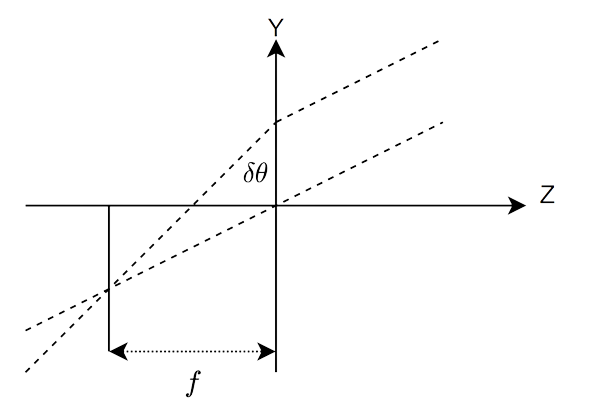
\includegraphics[width=0.4\linewidth]{images/focalization.png}
\end{figure}
In the image, we observe two rays: one passing through the center of the lens and another passing through a different point but remaining parallel to the first ray. 
Consequently, we can make the following observations:
\begin{itemize}
    \item When $Y = 0$, the ray experiences no deviation and continues without being deflected.
    \item Using the relationship $Y=f\cdot\delta\theta$, we can determine the focal length of the lens as follows: $f=\dfrac{1}{(n-1)\left(\dfrac{1}{\rho_1}+\dfrac{1}{\rho_2}\right)}$. 
\end{itemize}
This implies that all parallel rays converge to a common point, the focal point denoted as $Z$. 
The distance of this focal point from the $Y$ axis is given by:
\[Z=-f\]